%% ---------------------------------------------------------------------------
%% proposal.tex
%%
%% Research Proposal, main document.
%%
%% ---------------------------------------------------------------------------
\documentclass[12pt,letterpaper]{article}
\usepackage[english]{babel}     % supports english, but default is
% \usepackage[spanish]{babel}
% include this if you want to import graphics files with /includegraphics

\usepackage{longtable}
\usepackage{ifpdf}
\usepackage[table]{xcolor}

\usepackage{anysize}
\marginsize{2.5cm}{2.5cm}{1cm}{1cm}
\usepackage{textcomp}
\usepackage{url}
\bibliographystyle{unsrt}
\usepackage{graphics}
\usepackage{amssymb}
\usepackage{graphicx}
%\usepackage{slashbox}
\usepackage[latin1]{inputenc}
\usepackage{tikz}
\usetikzlibrary{arrows,positioning}
% Color and strikethrough



\usepackage{color}
\usepackage{soul}

\usepackage{array}
\usepackage{makecell}

\usepackage{sectsty}
\allsectionsfont{\sffamily}

\definecolor{dblue}{RGB}{0,102,153}
\newcommand{\dB}[1]{\textcolor{dblue}{\textbf{#1}}}



\setlength{\parskip}{1em}

% Nombre del Estudiante
\newcommand{\scriptAuthor}{Daniel Moya S�nchez}

% T��tulo de la tesis
\newcommand{\scriptTitle}{Project Plan} 


% Keywords
\newcommand{\scriptKeywords}{key, words, ...}

% Para el PDF (cambiar si se desea otras cosas a lo indicado arriba
\newcommand{\pdfAuthor}{\scriptAuthor}
\newcommand{\pdfTitle}{\scriptTitle} 
\newcommand{\pdfKeywords}{\scriptKeywords}


\tikzset{
    mynode/.style={rectangle,rounded corners,draw=black, top color=white, bottom color=yellow!50,very thick, inner sep=1em, minimum size=3em, text centered},
    myarrow/.style={->, >=latex', shorten >=1pt, thick},
    mylabel/.style={text width=7em, text centered} 
} 

\begin{document}
 
 \graphicspath{{./}{./fig/}}

 %% ---------------------------------------------------------------------------
%% titlepage.tex
%%
%% Title page
%%
%% ---------------------------------------------------------------------------

\thispagestyle{empty} 

\begin{center}

\textsc{\LARGE Instituto Tecnol\'ogico de Costa Rica} \\
\textsc{\Large Computer Engineering Academic Area}

\textsc{\Large Proyecto de Dise\~no en Ingenier\'ia en Computadores}


\par\vspace{20mm}

\includegraphics[scale=0.25]{logoTEC}

\par\vspace*{\fill}

{\LARGE\bf{\textsf{ \Huge \scriptTitle}}}

\par\vspace*{\fill}

%Master Thesis {\sf Proposal} \\ 
%in fulfillment of the requirements for the degree of
%Plan de Proyecto
%Master of Science in Electronics Engineering \\
%Emphasis on Embedded Systems

%\par\vspace{20mm}

\textsc{\Large \scriptAuthor}

\vspace*{\fill}

{\today}

\end{center}
\newpage 
\cleardoublepage  


%  \tableofcontents

 \clearpage

% El nombre del proyecto es preciso, conciso y no ambiguo
\section{Name of the project}

Design of Application Specific Instruction Set Processors (ASIPs) for Approximate Computing


% Se identifica claramente la instituci�n donde se realizar� el proyecto
\section{Name of the institution}

Chair for Embedded System (CES), Kalrsruhe Instituteof Technology (KIT), Germany, and 
Laboratorio Sistemas Embebidos y Electr�nica Digital
(SEED-Lab) del Instituto Tecnol�gico de Costa Rica



% Se identifica claramente qu� informaci�n se puede publicar, qu�
% informaci�n se puede compartir de manera limitada y qu�
% informaci�n se puede compartir si se firma un acuerdo de
% confidencialidad.
\section{Confidentiality requirements}

Due to the academic nature of the project, there are no confidentiality requirements, however,
there will not be published results during the development of the project but until the end of the work.




% El problema se describe de manera detallada, identificando los
% antecedentes, el contexto, usuarios, restricciones as� como otros
% aspectos relevantes para la resoluci�n del mismo.

% OPCIONAL: Se presenta una descripci�n del estado del arte de
% las investigaciones sobre el tema en cuesti�n.
\section{Problem description}


Dise�ar ASIPs aproximados para un conjunto de aplicaciones tolerantes a
errores.

Design Compiler and Prime Time, Synopsys

ModelSim, Mentor Graphics

ISE, Xilinx + tarjeta Virtex-IV/V

ASIPMeister

CoSy compiler



\section{Objectives}

% El objetivo general es directamente trazable al problema planteado, es claro, conciso.
\subsection{General objectives}
To explore the design of Application-Specific Instruction
Set Processors (ASIP) to be used in error tolerant applications.




% Los objetivos espec�ficos son suficientes y consistentes con el
% objetivo general
\subsection{Specific objectives}

The project has the following specific objectives:
\begin{enumerate}
 \item To select 3 error tolerant applications to be evaluated. 
 
 \item To develop at least 3 instances of approximated hardware for tolerant error sections for each of the selected applications. 
 
 
 \item To develop ASIPs configurations using specific approximated instruction.
 

 \item To evaluate, with the use of approximated instructions, a set of applications in terms of execution time, 
 area and power consumption vs the error achieved for the approximated ASIP.
 

\end{enumerate}



% La identificaci�n de los involucrados y sus relaciones con el
% proyecto es detallada. Las relaciones se describen en detalle,
% se�alando cu�l es el inter�s del involucrado.
\section{Project stakeholders}

Since this is an investigation project, there are only a few stakeholders, which are described below:

\begin{itemize}
 \item Jorge Castro: He is the supervisor of the project, has the general idea about the project itself and guides the course of it. 
 He wants to create new knowledge with the use of ASIPs, so that this area grows and future processes of creating approximated applications
 become more automated. 
 
 \item Sajjad Hussain: He works with Jorge Castro on the general guidance of the project, helps with any issue on the server in Germany
 so that the process of using the software platform (ASIPMeister, Dlxsim and other tools) remains smooth and clear. He has the same interest
 as Jorge Castro with the project. 
 
 \item Jeferson Gonz�lez: He is the supervisor in ITCR, helps with any resource assignation of whether space or resources (like the hardware platform)
 as the person in charge of the SEED laboratory.
 
\end{itemize}



% Se presenta una descripci�n de la soluci�n propuesta en
% correspondencia con el problema planteado y los objetivos.
% Se utilizan diagramas de bloques u otra informaci�n que permita
% visualizar la estrategia de soluci�n al problema planteado.

% OPCIONAL: Se pressentan varias alternativas de soluci�n a estudiar.
\section{Solution description}

\begin{figure}
\centering
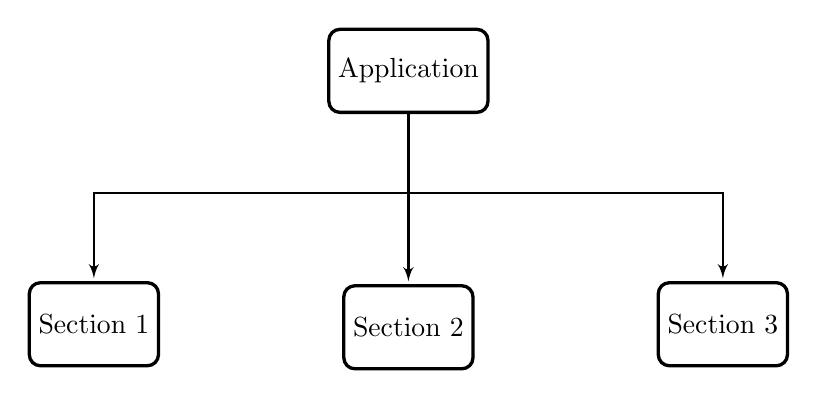
\begin{tikzpicture}[node distance=1cm, auto]  
\tikzset{
    mynode/.style={rectangle,rounded corners,draw=black, very thick, minimum size=3em, text centered},
    myarrow/.style={->, >=latex', shorten >=1pt, thick},
    mylabel/.style={text width=7em, text centered} 
}  
\node[mynode] (manufacturer) {Application};  
\node[mynode, below left =3cm of manufacturer] (section1) {Section 1}; 
\node[mynode, below=2.16cm of manufacturer] (section2) {Section 2};
\node[mynode, below right=3cm of manufacturer] (section3) {Section 3};



\draw[myarrow] (manufacturer.south)  -- ++(0,-1) -|  (section1.north);
\draw[myarrow] (manufacturer.south)   -|  (section2.north);
\draw[myarrow] (manufacturer.south)  -- ++(0,-1) -|  (section3.north); 
 
\end{tikzpicture} 
\medskip
\caption{Structure of the Market} 
\end{figure}



% Los entregables con consistentes con los objetivos del proyecto y
% con los productos de un proyecto de ingenier�a de software para
% efectos de desarrollo posterior o mantenimiento.
% Los entregables tienen un identificador �nico.
% Los entregables deben incluir:
%	- Documento de Requerimientos
%	- Documento de Dise�o
%	- Plan de pruebas/Resultados de las preubas
%	- Otra documentaci�n relevante: instrucciones de compilaci�n,
% manuales de instalaci�n, manual de usuario etc.
\section{Deliverables and criteria of acceptance}

The expected deliverables are the following:
\begin{table}
\begin{center}
\caption{Deliverables with the corresponding criteria of acceptance}
\begin{tabular}{ |c|c|c| } 
 \hline
Name & Description & Criteria of acceptance \\
 \hline
 Requirement 1.1 & Instances of approximated hardware & [criterio] \\ 
 Requirement 2.1 & Configuration of approximated ASIPs & [criterio] \\ 
 Requirement 3.1 & Data of execution time, area and power & [criterio] \\ %Plan de prueba
 Requirement 3.2 & Comparison and analysis of the obtained results & [criterio] \\ %Plan Prueba
 \hline
\end{tabular}
\label{tab:del}
\end{center}
\end{table}



% Las cuatro �reas analizadas (personal, herramientas, procesos,
% insumos) son analizadas en detalle, identificando los riesgos m�s
% sobresalientes para cada una de esas �reas. Para cada riesgo se
% indica la probabilidad y el impacto para el proyecto.
\section{Risky analysis}
\begin{table}
\begin{center}
\caption{Risk analysis}
\begin{tabular}{ | c | c | c | c | } 
 \hline
 Risk & \makecell{Probability of \\ occurrence} & \makecell{Impact \\ (hours)} & \makecell{Risk exposure \\ (hours)} \\
 \hline
  \makecell{Illness or any special medical condition} & 0.5 & 8 & 4 \\ 
 \makecell{General server errors (missing files, \\ permissions restrictions, etc)}   & 0.6 & 24 & 14.4 \\
 \makecell{Delays when acquiring the hardware equipment}   & 0.25 & 8 & 2 \\
 \hline
\end{tabular}
\label{tab:risk}
\end{center}
\end{table}



% Las actividades propuestas son consistentes con los objetivos
% espec�ficos.
% Las estimaciones de esfuerzos son proporcionales con la
% complejidad o el tama�o de las mismas.
% Se asigna un identificador �nico (c�digo) a cada actividad.
\section{Activities and effort budget}

The table \ref{tab:act} takes in consideration a total of 216 engineering hours. 

\begin{table}
\begin{center}
\caption{Activities and effort budget}
\begin{tabular}{ | c | c | c | c | c | } 
 \hline
 ID  &Activity & \makecell{Engineering \\ hours} & \makecell{Risk reserve \\ (hours)} & \makecell{Total \\ (hours)} \\
 \hline
 001 & \makecell{Get to know the software platform} & 24 & 2 & 26 \\
 \hline
\end{tabular}
\label{tab:act}
\end{center}
\end{table}


% El cronograma incluye todas las actividades y las mismas no
% guardan una consistecia l�gica para la construcci�n de los
% entregables.
% Se incluyen hitos para los entregables m�s sobresalientes.
% El nivel de granularidad de las actividades ofrece suficiente detalle.
% Al menos una actividad por semana.
\section{Schedule}

\begin{table}
\begin{center}
\caption{Schedule for the whole project}
\begin{tabular}{ | c | c | c | c | c | c | c | c | c | c | c | c | c | c | c | c | c |} 
 \hline
   & \multicolumn{16}{|c|}{Week} \\
 \hline
 Activity & 1 & 2 & 3 & 4 & 5 & 6 & 7 & 8 & 9 & 10 & 11 & 12 & 13 & 14 & 15 & 16 \\ \hline
 \makecell{Reading the corresponding \\ literature about the \\ project and understanding \\ the general idea of ASIPs}
 & \cellcolor[HTML]{AA0044}  &  &  &  &  &  &  &  &  &  &  &  &  &  &  &  \\ \hline
 \makecell{Execution of the laboratory \\ script to get  to know \\ the software tools like \\ ASIPMeister, Dlxsim, etc}
 & \cellcolor[HTML]{AA0044}  & \cellcolor[HTML]{AA0044}  &  &  &  &  &  &  &  &  &  &  &  &  &  &  \\ \hline
 \end{tabular}
\label{tab:schd}
\end{center}
\end{table}


% Referencias del Background y el Related Work
\bibliographystyle{sty/plainurl}
\bibliography{references}



\end{document}

